
\documentclass{article}
\usepackage{graphicx} % Required for inserting images
\usepackage{fancyhdr} % Required for header and footer configuration
\usepackage[a4paper, margin=2.5cm, left=1.5cm, right=1.5cm, bottom=4cm]{geometry} % Required for setting page margins
\usepackage[T1]{fontenc}
\usepackage[default,oldstyle,scale=1]{opensans} % Utilizzo del font Open Sans
\usepackage{lipsum}
\usepackage{makeidx}
\usepackage{booktabs}
\usepackage{tabularray}
\usepackage[colorlinks=true, linkcolor=black, urlcolor=blue, citecolor=blue]{hyperref}
\usepackage{tabularx}
\usepackage{makecell}
\usepackage{enumitem} % Pacchetto per la personalizzazione degli elenchi
\usepackage{booktabs}
\usepackage{subcaption}
\usepackage{pgfplots}
\usepgfplotslibrary{dateplot} % Per gestire gli assi con date

% Configure header and footer for the first page
\fancypagestyle{firstpage}{
    \fancyhf{} % Clear header and footer
    \renewcommand{\headrulewidth}{0pt} % Remove header rule line
    \lhead{} % Header on the left
    \chead{} % Header in the center
    \rhead{} % Header on the right
    \lfoot{} % Footer on the left
    \cfoot{\vspace{5pt}\\\hrulefill\\\vspace{10pt}\textbf{BeeLive}\\Gruppo 21} % Footer in the center
    \rfoot{\vspace{32.5pt}\\\thepage} % Footer on the right
}

% Configure header and footer for non-plain pages (second page onwards)
\fancypagestyle{nonplain}{
    \fancyhf{} % Clear header and footer
    \lhead{} % Header on the left
    \chead{} % Header in the center
    \rhead{
\includegraphics[width=2cm]{Images/BeeLive-Logo.png}\\\vspace{2pt}} % Header on the right
    \lfoot{} % Footer on the left
    \cfoot{\vspace{5pt}\\\hrulefill\\\vspace{10pt}\textbf{BeeLive}\\Gruppo 21} % Footer in the center
    \rfoot{\vspace{32.5pt}\\\thepage} % Footer on the right
}

% Adjust vertical space between header and text                                    
\setlength{\headsep}{65pt} 
% Adjust vertical space between text and footer
\setlength{\footskip}{0pt} 

\title{
\includegraphics[width=0.75\textwidth]{Images/BeeLive-Logo.png}\\\vspace{100pt}
\LARGE{\textbf{BeeLive\\Deliverable 2}}}
\author{Gruppo 21:\\
Cipriani Pietro, 226959\\
Orlando Dennis, 227688\\
Ziviani Elia, 228172}
\date{22 Aprile 2024}

\makeindex % Indica che vogliamo creare un indice

\begin{document}

\maketitle
\thispagestyle{firstpage} % Apply firstpage style to the first page
\clearpage

\pagestyle{nonplain} % Apply non-plain style to subsequent pages

\renewcommand{\contentsname}{Indice}
\tableofcontents

\clearpage

\section{Revisione}
Sono state apportate delle modifiche alla struttura del progetto definita nei precedenti delivareble. Queste modifiche sono così descritte: 

\subsubsection{Classe Evento e ausiliarie}
A seguito vi è il diagramma UML della classe \texttt{Evento} modificata; abbiamo modificato la gestione dei sottoeventi e usato una struttura "NullableTimeRange" ausiliaria, nonchè inserito un livello di rischio.\\
\begin{center}\includegraphics[width=0.735\textwidth]{Images/revisione\_evento.png}\end{center}

\section{Introduzione}

\subsection{Componenti del gruppo}
\begin{itemize}
    \item Cipriani Pietro, matricola 226959, \lbrack\href{https://github.com/pietrocipriani}{github profile}\rbrack
    \item Orlando Dennis, matricola 227688, \lbrack\href{https://github.com/dennisorlando}{github profile}\rbrack
    \item Ziviani Elia, matricola 228172, \lbrack\href{https://github.com/ELI20ZIVI}{github profile}\rbrack
\end{itemize}

\subsection{Scopo del progetto}

Lo scopo del progetto 'BeeLive' è quello di risolvere il problema riguardante la difficoltà nel reperire informazioni riguardanti gli eventi che influenzano la viabilità all'interno del Comune di Trento. Prevediamo un sistema informativo, dedicato agli utenti cittadini, che mostri visualmente le variazioni della viabilità in città, informando gli stessi di eventuali modifiche che potrebbero colpirli direttamente.

\subsection{Link utili}
Il primo link fornito è quello della repository github. La repository è stata creata appena il corso è cominciato, infatti inizialmente è risultata utile al fine di scrivere in modo collaborativo i primi deliverable.\\
E' stato deciso di integrare in questa repository anche le fasi di sprint in quanto come team riteniamo utile la possibilità di accedere alla documentazione redatta nei primi due deliverable.\\
La repository è accessibile al seguente link: \href{https://github.com/ELI20ZIVI/BeeLive/}{Repository GitHub}\\ \\
Il secondo link fornito è quello di Apiary. Apiary è uno strumento che permette di creare e documentare in modo molto accurato e approfontido le API utilizzate nel progetto.\\
Il link di Apiary è il seguente: \href{https://beelive.docs.apiary.io/#}{Link Apiary}\\

\clearpage

\section{Sezione generale}

\subsection{Strategia di Branching}

Per lo sviluppo dell'applicativo è stato evitato l'approccio "Master only": nonostante la piccola dimensione del team, la creazione ed utilizzo di un unico branch principale, \textit{main}, avrebbe comunque causato problemi di collaborazione e conflitti nel momento in cui avremmo lavorato contemporaneamente a stesse sezioni del progetto.\\

\noindent
Per aumentare la modulabilità e la scalabilità del progetto, abbiamo infatti adottato la strategia di branching prevedente la creazione di un 'branch' separato per ogni specifica feature del progetto, con un branch \textit{develop} intermedio.\\

\noindent
L'integrazione di una feature specifica avviene attraverso il merging del branch di quest'ultima nel precedentemente citato \textit{develop}; tale operazione è ammessa solamente da un diverso componente del gruppo, il cui compito sarà quello di assicurarsi che il modulo rispetti tutti i punti della "Definition of Done" definita dal team. \\

\noindent
Dato il branch \textit{develop}, definito come ambiente di lavoro in cui i membri del team lavorano e accumulano modifiche, una volta che ne sono accumulate abbastanza (e giudicato lo stato del progetto per intero come 'stabile' e 'shippable') verrà effettuato il merge di questa branch nel principale \texttt{main}, come operazione di 'release'. \\

\noindent
Tramite questo approccio puntiamo ad incrementare la collaborazione tra i membri del team, ridurre i conflitti e le inconsistenze nel codice, facilitare la gestione delle diverse attività in corso e mantenere inoltre una mappatura di tutte le diverse modifiche e progressi del progetto, mantenendo ben strutturata la storia del codice.\\

Segue una lista dei branch utilizzati per lo sviluppo del progetto; da notare che molte di queste branches sono state eliminate una volta integrate in \texttt{develop}, per cui su github potrebbero non apparire.

\subsubsection{\texttt{main}}
Il branch principale del progetto, in cui vengono integrate tutte le funzionalità completate e testate.\\
Tutte le funzionalita' all'interno di questo branch sono considerate terminate e funzionanti, pronte per essere rilasciate.\\
In questa branch abbiamo direttamente modificato e aggiornato i 'deliverable', prima di creare una branch \textit{deliverable} appositamente dedicata alla stesura di questi documenti.

\subsection{\texttt{deliverable}}
Branch dedicato alla stesura dei vari deliverable.

\subsubsection{\texttt{develop}}
Il branch di sviluppo del progetto, in cui vengono integrate tutte le funzionalità completate e testate.\\
Non e' pensato propriamente come il branch in cui vengono rilasciate le funzionalita' ma piuttosto come un branch di supporto per il branch principale, infatti in questo branch vengono prima caricate le funzionalita' dagli altri branch specifici e successivamente testate.\\
Una volta che sono considerate funzionanti sono quindi integrate nel branch principale.

\subsubsection{\texttt{ma\_screen}}
Branch dedicato alla creazione delle schermate dell'applicativo mobile, i.e. tutte le schermate che l'utente visualizzera' durante l'utilizzo dell'applicativo.\\
Questo branch è stato integrato in \texttt{ma\_client} in quanto sua dipendenza.

\subsubsection{\texttt{ma\_client}}
Branch dedicato allo sviluppo del client mobile, i.e. l'applicazione mobile utilizzata dagli utenti comuni (autenticati e non) che intendono visualizzazione le criticita' presenti in citta'.\\
Il branch, una volta concluso lo sviluppo dell'applicativo, e' stato integrato nel branch \texttt{develop} per i test in associata con tutti gli altri moduli.

\subsubsection{\texttt{ws-fetch-eventi}}
Branch dedicato allo sviluppo del webserver pubblico, i.e. il webserver in cui sono stati implementati gli endpoint API dedicati al fetching di eventi ad opera dell'applicativo mobile.\\
\\
Una volta che il modulo e' stato completato, e' stato integrato nel branch \texttt{develop} per i test con tutti gli altri moduli.


\subsubsection{\texttt{ws-insert-event}}
Branch dedicato allo sviluppo del webserver gestionale, i.e. il webserver in cui sono stati implementati gli endpoint API dedicati all'inserimento degli eventi all'interno del sistema ad opera dell'applicativo desktop. \\
Utile allo sviluppo del modulo utilizzato dall'applicativo desktop per l'inserimento delle criticita' in citta'.
Una volta che il modulo e' stato completato, e' stato integrato nel branch \texttt{develop} per i test con tutti gli altri moduli.\\
Delle versioni intermedie di questa branch sono state usate da altre branches, in particolare da \texttt{da\_desktop}, in quanto necessaria per effettuare il testing di quest'ultima.


\subsubsection{\texttt{da\_frontend}}
Branch dedicato allo sviluppo dell'applicativo desktop, quindi l'applicativo utilizzato dagli utenti autorizzati (del comune e non) per inserire a sistema le criticità (eventi) presenti in città.\\
Una volta concluso lo sviluppo del modulo frontend, il branch è stato integrato nel branch \texttt{develop} e integrato con gli altri moduli.

\subsubsection{\texttt{preview}}
Branch dedicato alla preview dell'interfaccia grafica dei due applicativi.\\
E' stato utilizzato al momento della prima presentazione del progetto per mostrare il lavoro svolto ai committenti e per ricevere feedback su eventuali modifiche da apportare.\\
Integra dei mockup delle varie interfacce, desktop e mobile, che andranno sviluppate.\\
Parte della preview è stata poi utilizzata in \texttt{da\_frontend} come punto di partenza per l'interfaccia,

\clearpage

\subsection{Product Backlog}
Nella pagina seguente vi è riportato il product backlog che abbiamo sviluppato per questo progetto. E' possibile notare una linea di demarcazione che limita inferiormente le entries selezionate per il primo sprint.

\begin{table}[!ht]
    \centering
    \renewcommand{\arraystretch}{1.3} % Imposta lo spazio verticale delle righe
    \begin{tabularx}{\textwidth}{| r | X | r | r |}
        \Xhline{2pt}
        \makecell{\textbf{Nome}} & \makecell{\textbf{User story}} & \makecell{\textbf{Priorità}} & \makecell{\textbf{Stima}} \\
        \Xhline{2pt}
        \makecell{Visualizzazione\\eventi in città} & \makecell{Da utente, voglio visualizzare la lista degli eventi in città} & \makecell{200} & \makecell{8}\\
        \hline
        \makecell{Aggiunta eventi\\da utente\\autorizzato} & \makecell{Da utente autorizzato, devo essere in grado di aggiungere degli eventi\\in modo da comunicare la loro presenza agli utenti} & \makecell{190} & \makecell{8}\\
        \hline
        \makecell{Registrazione e\\accesso all'\\app mobile} & \makecell{Da utente, voglio avere la possibilità di accedere ad una\\visualizzazione e descrizione più dettagliata di un evento in modo da\\conoscere meglio le specifiche di tale evento} & \makecell{180} & \makecell{8}\\
        \hline
        \makecell{Visualizzazione\\criticità\\su mappa} & \makecell{Da utente, voglio visualizzare su una cartina le zone colpite dai diversi\\eventi, in modo da capire visivamente se in una zona che mi\\interessa vi è un evento attivo} & \makecell{170} & \makecell{6}\\
        \hline
        \makecell{Accesso alle\\criticità e ai\\loro dettagli} & \makecell{Da utente, voglio essere in grado di visualizzare la lista\\delle criticità presenti in città} & \makecell{160} & \makecell{8}\\
        \Xhline{2pt}
        \makecell{Impostazione\\categorie\\d'interesse\\per gli eventi} & \makecell{Da utente, voglio essere in grado di impostare le categorie di eventi\\alle quali io sono interessato, in modo che la lista di eventi visibile\\dall'applicazione contenga solamente gli eventi che mi interessano,\\e in modo che io non venga notificato di alcun evento\\che io non ritenga appartenere ad una categoria interessante} & \makecell{100} & \makecell{5}\\
        \hline
        \makecell{Impostazione\\zone\\d'interesse} & \makecell{Da utente, voglio essere in grado di impostare delle zone di interesse,\\in modo che io venga notificato di qualsiasi evento che insorga\\in una di queste zone} & \makecell{90} & \makecell{7}\\
        \hline
        \makecell{Visualizzazione\\eventi\\di competenza} & \makecell{Da utente autorizzato, devo essere in grado di visualizzare gli eventi\\di mia competenza, in modo da sapere quali eventi sono stati creati e\\monitorare il loro stato} & \makecell{80} & \makecell{5}\\
        \hline
        \makecell{Modifica\\eventi} & \makecell{Da utente autorizzato, devo essere in grado di modificare degli eventi\\in modo da evitare errori comunicativi} & \makecell{75} & \makecell{2}\\
        \hline
        \makecell{Accesso\\account\\utente} & \makecell{Da utente registrato, voglio essere in grado di poter accedere al\\mio account in modo da poter riottenere le aree di interesse e\\le impostazioni che ho precedentemente salvato} & \makecell{70} & \makecell{3}\\
        \hline
        \makecell{Visualizzazione\\eventi\\di categorie\\di interesse} & \makecell{Da utente, voglio essere in grado di visualizzare solo\\eventi di categorie di interesse} & \makecell{60} & \makecell{3}\\
        \hline
        \makecell{Selezione\\percorso} & \makecell{Da utente, voglio essere in grado di selezionare un percorso a partire\\da dei waypoint, per impostare dei percorsi di interesse} & \makecell{40} & \makecell{2}\\
        \hline
        \makecell{Eliminazione\\eventi} & \makecell{Da utente autorizzato, devo essere in grado di eliminare degli eventi} & \makecell{40} & \makecell{2}\\
        \hline
    \end{tabularx}
    \caption{Product backlog}
\end{table}

\clearpage

\subsection{Definition of "Done"}
La seguente 'Definition of Done' è basata su una valutazione collettiva che ha preso in considerazione  diversi fattori riguardanti la qualità del lavoro, non ignorando però la fattibilità e la realizzabilità di questi.\\
I criteri inclusi nella nostra 'Definition of Done' definita per il progetto sono i seguenti:
\begin{itemize}
	\item \textbf{Funzionalità}: le funzionalità che il codice implementa devono soddisfare appieno l'usecase / gli usecase associati al codice.
    \item \textbf{Codice}: Il codice deve essere revisionato e la sua correttezza / adeguatezza approvata da almeno un altro membro del team.
    \item \textbf{Test}: Il codice deve essere adeguatamente coperto da test unitari, di integrazione e funzionali, che devono essere scritti e superati con successo. Un adeguato numero di questi test deve essere scritto da membri diversi.
    \item \textbf{Documentazione}: Il codice e le funzionalità implementate devono essere adeguatamente documentati. Questo giudizio di adeguatezza deve essere dato da almeno un altro membro del team.
    \item \textbf{Build e Deployment}: Il codice deve integrarsi con successo nella build principale e la sua inclusione nella build principale non deve assolutamente far fallire dei test, nel caso in cui quest'ultimi venivano correttamente superati priva dell'inclusione.
    \item \textbf{Performance}: le funzionalità e il codice introdotti non devono causare visibili degradi alle performance di nessun elemento del progetto.
    \item \textbf{Conformità}: Il prodotto deve essere conforme alle normative legali e agli standard di sicurezza e qualità specifici del settore.
\end{itemize}

\clearpage

\section{Sezione Sprint \#1}

\subsection{Goal dello sprint}
Lo scopo di questo primo sprint è stato quello di creare un prototipo funzionante dell'applicazione, che presenti le funzionalità core del nostro progetto e che quindi includa queste funzionalità:
\begin{enumerate}
\item Possibilità da parte di un utente autorizzato di aggiungere eventi al sistema
\item Possibilità da parte degli utenti di visualizzare gli eventi aggiunti
\end{enumerate}
È stato dunque necessario lavorare, oltre al 'backend', anche allo sviluppo sia dell'applicativo mobile dedicato ad utenti comuni che all'applicativo desktop, dedicato agli utenti autorizzati.

Scendendo più in dettaglio, le funzionalità che abbiamo deciso di includere nello sprint sono, per quanto riguarda la parte mobile, la visualizzazione degli eventi disponibili e dei loro relativi dettagli, anche includendo la visualizzazione su mappa.\\
E' stato inoltre inserita, anche se con bassa priorità, la funzionalità riguardante la possibilità di effettuare l'autenticazione (da parte degli utenti comuni) per poter salvare le proprie impostazioni e preferenze sul database.\\
Per quanto riguarda la parte desktop, ci siamo limitati a rendere possibile l'aggiunta degli eventi al sistema, rimandando l'autenticazione degli utenti autorizzati a sprint successivi.

\subsection{Sprint Planning}
E' riportato il product backlog per ogni user story trattata in questo primo sprint, con tutte le informazioni relative ai task da completare, a chi sono assegnati e la loro priorità.\\
\subsubsection{Aggiunta eventi da utente autorizzato}
\textbf{User story}: Da utente autorizzato, devo essere in grado di aggiungere degli eventi in modo da comunicare la loro presenza agli utenti.\\

\textbf{Product backlog}
\begin{table}[htbp]
    \centering
    \renewcommand{\arraystretch}{1.3} % Imposta lo spazio verticale delle righe
    \begin{tabularx}{\textwidth}{| X | r | r | r | r |}
        \Xhline{2pt}
        \makecell{\textbf{Nome}} & \makecell{\textbf{User story}} & \makecell{\textbf{Cosa fare}} & \makecell{\textbf{Assegnazione}} & \makecell{\textbf{Stima}} \\
        \Xhline{2pt}
        \makecell{Aggiunta\\eventi\\da utente\\autorizzato} & \makecell{Da utente autorizzato,\\devo essere in grado di\\aggiungere degli eventi in\\modo da comunicare la\\loro presenza agli utenti} & \makecell{Creazione screen (DA)\\Creazione metodo del client (DA)\\Creazione API endpoint (WS)\\Creazione metodo del DAO (WS)\\Creazione modulo gestione mappa\\Creazione event manager (WS)\\Creazione test (WS)\\Creazione test (DA)} & \makecell{Dennis Orlando\\Dennis Orlando\\Dennis Orlando\\Pietro Cipriani\\Pietro Cipriani\\Pietro Cipriani\\Elia Ziviani\\-} & \makecell{5\\3\\4\\4\\3\\2\\4\\4} \\
        \hline
    \end{tabularx}
    \caption{Product backlog user story 1}
\end{table}

\clearpage

\textbf{Progresso}
\begin{table}[htbp]
    \centering
    \renewcommand{\arraystretch}{1.3} % Imposta lo spazio verticale delle righe
    \begin{tabularx}{\textwidth}{| X | r | r | r | r | r | r | r | r | r | r | r | r | r | r | r | r |}
        \Xhline{2pt}
        \makecell{\textbf{Nome}} & \makecell{\textbf{1}} & \makecell{\textbf{2}} & \makecell{\textbf{3}} & \makecell{\textbf{4}} & \makecell{\textbf{5}} & \makecell{\textbf{6}} & \makecell{\textbf{7}} & \makecell{\textbf{8}} & \makecell{\textbf{9}} & \makecell{\textbf{10}} & \makecell{\textbf{11}} & \makecell{\textbf{12}} & \makecell{\textbf{13}} & \makecell{\textbf{14}} & \makecell{\textbf{15}} & \makecell{\textbf{16}} \\
        \Xhline{2pt}
        \makecell{Creazione screen (DA)} & \makecell{5} & \makecell{5} & \makecell{5} & \makecell{5} & \makecell{5} & \makecell{5} & \makecell{5} & \makecell{5} & \makecell{4} & \makecell{4} & \makecell{3} & \makecell{2} & \makecell{1} & \makecell{0} & \makecell{0} & \makecell{0} \\
        \hline
        \makecell{Creazione metodo del client (DA)} & \makecell{3} & \makecell{3} & \makecell{3} & \makecell{3} & \makecell{3} & \makecell{3} & \makecell{3} & \makecell{3} & \makecell{3} & \makecell{3} & \makecell{2} & \makecell{1} & \makecell{1} & \makecell{0} & \makecell{0} & \makecell{0} \\
        \hline
        \makecell{Creazione API endpoint (WS)} & \makecell{4} & \makecell{4} & \makecell{4} & \makecell{4} & \makecell{4} & \makecell{4} & \makecell{3} & \makecell{3} & \makecell{3} & \makecell{1} & \makecell{1} & \makecell{0} & \makecell{0} & \makecell{0} & \makecell{0} & \makecell{0} \\
        \hline
        \makecell{Creazione metodo del DAO (WS)} & \makecell{4} & \makecell{4} & \makecell{4} & \makecell{4} & \makecell{4} & \makecell{4} & \makecell{4} & \makecell{0} & \makecell{0} & \makecell{0} & \makecell{0} & \makecell{0} & \makecell{0} & \makecell{0} & \makecell{0} & \makecell{0} \\
        \hline
        \makecell{Creazione modulo gestione mappa} & \makecell{3} & \makecell{3} & \makecell{3} & \makecell{3} & \makecell{3} & \makecell{0} & \makecell{0} & \makecell{0} & \makecell{0} & \makecell{0} & \makecell{0} & \makecell{0} & \makecell{0} & \makecell{0} & \makecell{0} & \makecell{0} \\
        \hline
        \makecell{Creazione event manager (WS)} & \makecell{2} & \makecell{0} & \makecell{0} & \makecell{0} & \makecell{0} & \makecell{0} & \makecell{0} & \makecell{0} & \makecell{0} & \makecell{0} & \makecell{0} & \makecell{0} & \makecell{0} & \makecell{0} & \makecell{0} & \makecell{0} \\
        \hline
        \makecell{Creazione test (WS)} & \makecell{4} & \makecell{4} & \makecell{4} & \makecell{4} & \makecell{4} & \makecell{4} & \makecell{4} & \makecell{4} & \makecell{4} & \makecell{4} & \makecell{4} & \makecell{4} & \makecell{4} & \makecell{4} & \makecell{4} & \makecell{4} \\
        \hline
        \makecell{Creazione test (DA)} & \makecell{4} & \makecell{4} & \makecell{4} & \makecell{4} & \makecell{4} & \makecell{4} & \makecell{4} & \makecell{4} & \makecell{4} & \makecell{4} & \makecell{4} & \makecell{4} & \makecell{4} & \makecell{4} & \makecell{4} & \makecell{4} \\
        \hline
    \end{tabularx}
    \caption{Progresso user story 1}
\end{table}

\subsubsection{Visualizzazione eventi e dettagli da utente mobile}
\textbf{User story}: Da utente, voglio avere la possibilità di accedere ad una visualizzazione e descrizione più dettagliata di un evento in modo da conoscere meglio le specifiche di tale evento.\\
\begin{table}[htbp]
    \centering
    \renewcommand{\arraystretch}{1.3} % Imposta lo spazio verticale delle righe
    \begin{tabularx}{\textwidth}{| X | r | r | r | r |}
        \Xhline{2pt}
        \makecell{\textbf{Nome}} & \makecell{\textbf{User story}} & \makecell{\textbf{Cosa fare}} & \makecell{\textbf{Assegnazione}} & \makecell{\textbf{Stima}} \\
        \Xhline{2pt}
        \makecell{Visualizzazione\\eventi\\e dettagli\\da utente\\mobile} & \makecell{Da utente, voglio avere\\la possibilità di accedere\\ad una visualizzazione e\\descrizione più dettagliata\\di un evento in modo da\\conoscere meglio le\\specifiche di tale evento} & \makecell{Creazione screen (DA)\\Creazione API endpoint (WS)\\Creazione metodo del client (DA)\\Creazione metodo del DAO (WS)\\Estensione Event Processor\\Creazione test (WS)\\Creazione test (DA)} & \makecell{-\\Dennis Orlando\\-\\Dennis Orlando\\Dennis Orlando\\Elia Ziviani\\-} & \makecell{4\\2\\2\\2\\2\\4\\4} \\
        \hline
    \end{tabularx}
    \caption{Product backlog user story 2}
\end{table}

\textbf{Progresso}
\begin{table}[htbp]
    \centering
    \renewcommand{\arraystretch}{1.3} % Imposta lo spazio verticale delle righe
    \begin{tabularx}{\textwidth}{| X | r | r | r | r | r | r | r | r | r | r | r | r | r | r | r | r |}
        \Xhline{2pt}
        \makecell{\textbf{Nome}} & \makecell{\textbf{1}} & \makecell{\textbf{2}} & \makecell{\textbf{3}} & \makecell{\textbf{4}} & \makecell{\textbf{5}} & \makecell{\textbf{6}} & \makecell{\textbf{7}} & \makecell{\textbf{8}} & \makecell{\textbf{9}} & \makecell{\textbf{10}} & \makecell{\textbf{11}} & \makecell{\textbf{12}} & \makecell{\textbf{13}} & \makecell{\textbf{14}} & \makecell{\textbf{15}} & \makecell{\textbf{16}} \\
        \Xhline{2pt}
        \makecell{Creazione screen (DA)} & \makecell{4} & \makecell{4} & \makecell{4} & \makecell{4} & \makecell{4} & \makecell{4} & \makecell{4} & \makecell{4} & \makecell{4} & \makecell{4} & \makecell{4} & \makecell{4} & \makecell{4} & \makecell{4} & \makecell{4} & \makecell{4} \\
        \hline
        \makecell{Creazione API endpoint (WS)} & \makecell{2} & \makecell{2} & \makecell{2} & \makecell{2} & \makecell{2} & \makecell{2} & \makecell{0} & \makecell{0} & \makecell{0} & \makecell{0} & \makecell{0} & \makecell{0} & \makecell{0} & \makecell{0} & \makecell{0} & \makecell{0}  \\
        \hline
        \makecell{Creazione metodo del client (DA)} & \makecell{2} & \makecell{2} & \makecell{2} & \makecell{2} & \makecell{2} & \makecell{2} & \makecell{2} & \makecell{2} & \makecell{2} & \makecell{2} & \makecell{2} & \makecell{2} & \makecell{2} & \makecell{2} & \makecell{2} & \makecell{2} \\
        \hline
        \makecell{Creazione metodo del DAO (WS)} & \makecell{2} & \makecell{2} & \makecell{2} & \makecell{2} & \makecell{2} & \makecell{2} & \makecell{0} & \makecell{0} & \makecell{0} & \makecell{0} & \makecell{0} & \makecell{0} & \makecell{0} & \makecell{0} & \makecell{0} & \makecell{0}  \\
        \hline
        \makecell{Estensione Event Processor} & \makecell{2} & \makecell{2} & \makecell{2} & \makecell{2} & \makecell{2} & \makecell{2} & \makecell{0} & \makecell{0} & \makecell{0} & \makecell{0} & \makecell{0} & \makecell{0} & \makecell{0} & \makecell{0} & \makecell{0} & \makecell{0}  \\
        \hline
        \makecell{Creazione test (WS)} & \makecell{4} & \makecell{4} & \makecell{4} & \makecell{4} & \makecell{4} & \makecell{4} & \makecell{4} & \makecell{4} & \makecell{4} & \makecell{4} & \makecell{4} & \makecell{4} & \makecell{4} & \makecell{4} & \makecell{4} & \makecell{4} \\
        \hline
        \makecell{Creazione test (DA)} & \makecell{4} & \makecell{4} & \makecell{4} & \makecell{4} & \makecell{4} & \makecell{4} & \makecell{4} & \makecell{4} & \makecell{4} & \makecell{4} & \makecell{4} & \makecell{4} & \makecell{4} & \makecell{4} & \makecell{4} & \makecell{4} \\
        \hline
    \end{tabularx}
    \caption{Progresso user story 2}
\end{table}

\subsubsection{Registrazione account utente mobile}
\textbf{User story}: Da utente voglio essere in grado di poter registrare un account in modo da poter salvare le mie impostazioni e le aree di interesse che io ho impostato.\\
\begin{table}[htbp]
    \centering
    \renewcommand{\arraystretch}{1.3} % Imposta lo spazio verticale delle righe
    \begin{tabularx}{\textwidth}{| X | r | r | r | r |}
        \Xhline{2pt}
        \makecell{\textbf{Nome}} & \makecell{\textbf{User story}} & \makecell{\textbf{Cosa fare}} & \makecell{\textbf{Assegnazione}} & \makecell{\textbf{Stima}} \\
        \Xhline{2pt}
        \makecell{Registrazione\\account\\utente\\mobile} & \makecell{Da utente voglio essere\\in grado di poter registrare\\un account in modo da\\poter salvare le mie\\impostazioni e le aree di\\interesse che io ho impostato} & \makecell{Creazione screen login (MA)\\Istanziazione casdoor\\Sincro preferenze locali (MA)\\Client: Gestione token (MA)\\Modifica API endpoints\\Creazione auth. SDK (WS)\\Creazione default AC policies\\Creazione tests(WS)\\Creazione tests(MA)} & \makecell{Pietro Cipriani\\Elia e Pietro\\-\\Pietro Cipriani\\Elia Ziviani\\-\\-\\Elia Ziviani\\-} & \makecell{4\\6\\4\\2\\4\\3\\3\\4\\4} \\
        \hline
    \end{tabularx}
    \caption{Product backlog user story 3}
\end{table}

\textbf{Progresso}
\begin{table}[htbp]
    \centering
    \renewcommand{\arraystretch}{1.3} % Imposta lo spazio verticale delle righe
    \begin{tabularx}{\textwidth}{| X | r | r | r | r | r | r | r | r | r | r | r | r | r | r | r | r |}
        \Xhline{2pt}
        \makecell{\textbf{Nome}} & \makecell{\textbf{1}} & \makecell{\textbf{2}} & \makecell{\textbf{3}} & \makecell{\textbf{4}} & \makecell{\textbf{5}} & \makecell{\textbf{6}} & \makecell{\textbf{7}} & \makecell{\textbf{8}} & \makecell{\textbf{9}} & \makecell{\textbf{10}} & \makecell{\textbf{11}} & \makecell{\textbf{12}} & \makecell{\textbf{13}} & \makecell{\textbf{14}} & \makecell{\textbf{15}} & \makecell{\textbf{16}} \\
        \Xhline{2pt}
        \makecell{Creazione screen login (MA)} & \makecell{4} & \makecell{4} & \makecell{4} & \makecell{4} & \makecell{4} & \makecell{4} & \makecell{4} & \makecell{4} & \makecell{4} & \makecell{4} & \makecell{4} & \makecell{4} & \makecell{4} & \makecell{4} & \makecell{4} & \makecell{4} \\
        \hline
        \makecell{Istanziazione casdoor} & \makecell{6} & \makecell{6} & \makecell{6} & \makecell{4} & \makecell{4} & \makecell{4} & \makecell{3} & \makecell{3} & \makecell{2} & \makecell{2} & \makecell{2} & \makecell{1} & \makecell{0} & \makecell{0} & \makecell{0} & \makecell{0} \\
        \hline
        \makecell{Sincro preferenze locali (MA)} & \makecell{4} & \makecell{4} & \makecell{4} & \makecell{4} & \makecell{4} & \makecell{4} & \makecell{4} & \makecell{4} & \makecell{4} & \makecell{4} & \makecell{4} & \makecell{4} & \makecell{4} & \makecell{4} & \makecell{4} & \makecell{4} \\
        \hline
        \makecell{Client: Gestione token (MA)} & \makecell{2} & \makecell{2} & \makecell{2} & \makecell{2} & \makecell{2} & \makecell{2} & \makecell{2} & \makecell{2} & \makecell{2} & \makecell{2} & \makecell{2} & \makecell{2} & \makecell{2} & \makecell{2} & \makecell{2} & \makecell{2} \\
        \hline
        \makecell{Modifica API endpoints} & \makecell{4} & \makecell{4} & \makecell{4} & \makecell{4} & \makecell{4} & \makecell{2} & \makecell{0} & \makecell{0} & \makecell{0} & \makecell{0} & \makecell{0} & \makecell{0} & \makecell{0} & \makecell{0} & \makecell{0} & \makecell{0} \\
        \hline
        \makecell{Creazione auth. SDK (WS)} & \makecell{3} & \makecell{3} & \makecell{3} & \makecell{3} & \makecell{3} & \makecell{3} & \makecell{3} & \makecell{3} & \makecell{3} & \makecell{3} & \makecell{3} & \makecell{3} & \makecell{3} & \makecell{3} & \makecell{3} & \makecell{3} \\
        \hline
        \makecell{Creazione default AC policies} & \makecell{3} & \makecell{3} & \makecell{3} & \makecell{3} & \makecell{3} & \makecell{3} & \makecell{3} & \makecell{3} & \makecell{3} & \makecell{3} & \makecell{3} & \makecell{3} & \makecell{3} & \makecell{3} & \makecell{3} & \makecell{3} \\
        \hline
        \makecell{Creazione tests(WS)} & \makecell{4} & \makecell{4} & \makecell{4} & \makecell{4} & \makecell{4} & \makecell{4} & \makecell{4} & \makecell{4} & \makecell{4} & \makecell{4} & \makecell{4} & \makecell{2} & \makecell{0} & \makecell{0} & \makecell{0} & \makecell{0} \\
        \hline
        \makecell{Creazione tests(MA)} & \makecell{4} & \makecell{4} & \makecell{4} & \makecell{4} & \makecell{4} & \makecell{4} & \makecell{4} & \makecell{4} & \makecell{4} & \makecell{4} & \makecell{4} & \makecell{4} & \makecell{4} & \makecell{4} & \makecell{4} & \makecell{4} \\
        \hline
    \end{tabularx}
    \caption{Progresso user story 3}
\end{table}

\clearpage

\subsubsection{Accesso alle criticità in città}
\textbf{User story}: Da utente voglio essere in grado di visualizzare la lista delle criticità presenti in città.\\
\begin{table}[htbp]
    \centering
    \renewcommand{\arraystretch}{1.3} % Imposta lo spazio verticale delle righe
    \begin{tabularx}{\textwidth}{| X | r | r | r | r |}
        \Xhline{2pt}
        \makecell{\textbf{Nome}} & \makecell{\textbf{User story}} & \makecell{\textbf{Cosa fare}} & \makecell{\textbf{Assegnazione}} & \makecell{\textbf{Stima}} \\
        \Xhline{2pt}
        \makecell{Accesso alle\\criticità in\\città} & \makecell{Da utente voglio essere\\in grado di visualizzare la\\lista delle criticità presenti\\in città} & \makecell{Istanziazione DB\\Creazione screen (MA)\\Creazione API endpoint (WS)\\Creazione metodo del DAO(WS)\\Creazione metodo del client(MA)\\Creazione event processor(WS)\\Creazione test(WS)\\Creazione test(MA)\\Istanziazione public server} & \makecell{Elia Ziviani\\Pietro Cipriani\\Dennis Orlando\\Dennis Orlando\\Pietro Cipriani\\Dennis Orlando\\Elia Ziviani\\-\\Elia Ziviani} & \makecell{2\\5\\4\\2\\2\\1\\5\\5\\-} \\
        \hline
    \end{tabularx}
    \caption{Product backlog user story 4}
\end{table}

\textbf{Progresso}
\begin{table}[htbp]
    \centering
    \renewcommand{\arraystretch}{1.3} % Imposta lo spazio verticale delle righe
    \begin{tabularx}{\textwidth}{| X | r | r | r | r | r | r | r | r | r | r | r | r | r | r | r | r |}
        \Xhline{2pt}
        \makecell{\textbf{Nome}} & \makecell{\textbf{1}} & \makecell{\textbf{2}} & \makecell{\textbf{3}} & \makecell{\textbf{4}} & \makecell{\textbf{5}} & \makecell{\textbf{6}} & \makecell{\textbf{7}} & \makecell{\textbf{8}} & \makecell{\textbf{9}} & \makecell{\textbf{10}} & \makecell{\textbf{11}} & \makecell{\textbf{12}} & \makecell{\textbf{13}} & \makecell{\textbf{14}} & \makecell{\textbf{15}} & \makecell{\textbf{16}} \\
        \Xhline{2pt}
        \makecell{Istanziazione DB} & \makecell{2} & \makecell{2} & \makecell{0} & \makecell{0} & \makecell{0} & \makecell{0} & \makecell{0} & \makecell{0} & \makecell{0} & \makecell{0} & \makecell{0} & \makecell{0} & \makecell{0} & \makecell{0} & \makecell{0} & \makecell{0} \\
        \hline
        \makecell{Creazione screen (MA)} & \makecell{5} & \makecell{2} & \makecell{2} & \makecell{2} & \makecell{1}  & \makecell{0} & \makecell{0} & \makecell{0} & \makecell{0} & \makecell{0} & \makecell{0} & \makecell{0} & \makecell{0} & \makecell{0} & \makecell{0} & \makecell{0}\\
        \hline
        \makecell{Creazione API endpoint (WS)} & \makecell{4} & \makecell{4} & \makecell{4} & \makecell{4} & \makecell{4} & \makecell{0} & \makecell{0} & \makecell{0} & \makecell{0} & \makecell{0} & \makecell{0} & \makecell{0} & \makecell{0} & \makecell{0} & \makecell{0} & \makecell{0} \\
        \hline
        \makecell{Creazione metodo del DAO(WS)} & \makecell{2} & \makecell{2} & \makecell{2} & \makecell{2} & \makecell{0} & \makecell{0} & \makecell{0} & \makecell{0} & \makecell{0} & \makecell{0} & \makecell{0} & \makecell{0} & \makecell{0} & \makecell{0} & \makecell{0} & \makecell{0} \\
        \hline
        \makecell{Creazione metodo del client(MA)} & \makecell{2} & \makecell{2} & \makecell{2} & \makecell{2} & \makecell{2} & \makecell{2} & \makecell{0} & \makecell{0} & \makecell{0} & \makecell{0} & \makecell{0} & \makecell{0} & \makecell{0} & \makecell{0} & \makecell{0} & \makecell{0} \\
        \hline
        \makecell{Creazione event processor(WS)} & \makecell{1} & \makecell{1} & \makecell{1} & \makecell{1} & \makecell{1} & \makecell{0} & \makecell{0} & \makecell{0} & \makecell{0} & \makecell{0} & \makecell{0} & \makecell{0} & \makecell{0} & \makecell{0} & \makecell{0} & \makecell{0} \\
        \hline
        \makecell{Creazione test(WS)} & \makecell{5} & \makecell{5} & \makecell{5} & \makecell{5} & \makecell{5} & \makecell{5} & \makecell{5} & \makecell{5} & \makecell{3} & \makecell{3} & \makecell{1} & \makecell{0}  & \makecell{0} & \makecell{0} & \makecell{0} & \makecell{0} \\
        \hline
        \makecell{Creazione test(MA)} & \makecell{5} & \makecell{5} & \makecell{5} & \makecell{5} & \makecell{5} & \makecell{5} & \makecell{5} & \makecell{5} & \makecell{5} & \makecell{5} & \makecell{5} & \makecell{5} & \makecell{5} & \makecell{5} & \makecell{5} & \makecell{5} \\
        \hline
        \makecell{Istanziazione public server} & \makecell{4} & \makecell{4} & \makecell{4} & \makecell{4} & \makecell{3} & \makecell{1} & \makecell{0} & \makecell{0} & \makecell{0} & \makecell{0} & \makecell{0} & \makecell{0} & \makecell{0} & \makecell{0} & \makecell{0} & \makecell{0} \\
        \hline
    \end{tabularx}
    \caption{Progresso user story 4}
\end{table}

\subsubsection{Visualizzazione criticità su mappa}
\textbf{User story}: Da utente voglio visualizzare su una cartina le zone colpite dai diversi eventi, in modo da capire visivamente se in una zona di mio interesse vi è un evento attivo.\\
\begin{table}[htbp]
    \centering
    \renewcommand{\arraystretch}{1.3} % Imposta lo spazio verticale delle righe
    \begin{tabularx}{\textwidth}{| X | r | r | r | r |}
        \Xhline{2pt}
        \makecell{\textbf{Nome}} & \makecell{\textbf{User story}} & \makecell{\textbf{Cosa fare}} & \makecell{\textbf{Assegnazione}} & \makecell{\textbf{Stima}} \\
        \Xhline{2pt}
        \makecell{Visualizzazione\\criticità\\su mappa} & \makecell{Da utente voglio\\visualizzare su una cartina\\le zone colpite dai diversi\\eventi, in modo da capire\\visivamente se in una zona\\di mio interesse vi è un\\evento attivo} & \makecell{Estensione screen (MA)\\Creazione tests (MA)} & \makecell{-\\-} & \makecell{3\\2} \\
        \hline
    \end{tabularx}
    \caption{Product backlog user story 5}
\end{table}

\clearpage

\textbf{Progresso}
\begin{table}[htbp]
    \centering
    \renewcommand{\arraystretch}{1.3} % Imposta lo spazio verticale delle righe
    \begin{tabularx}{\textwidth}{| X | r | r | r | r | r | r | r | r | r | r | r | r | r | r | r | r |}
        \Xhline{2pt}
        \makecell{\textbf{Nome}} & \makecell{\textbf{1}} & \makecell{\textbf{2}} & \makecell{\textbf{3}} & \makecell{\textbf{4}} & \makecell{\textbf{5}} & \makecell{\textbf{6}} & \makecell{\textbf{7}} & \makecell{\textbf{8}} & \makecell{\textbf{9}} & \makecell{\textbf{10}} & \makecell{\textbf{11}} & \makecell{\textbf{12}} & \makecell{\textbf{13}} & \makecell{\textbf{14}} & \makecell{\textbf{15}} & \makecell{\textbf{16}} \\
        \Xhline{2pt}
        \makecell{Estensione screen (MA)} & \makecell{3} & \makecell{3} & \makecell{3} & \makecell{3} & \makecell{3} & \makecell{3} & \makecell{3} & \makecell{3} & \makecell{3} & \makecell{3} & \makecell{3} & \makecell{3} & \makecell{3} & \makecell{3} & \makecell{3} & \makecell{3} \\
        \hline
        \makecell{Creazione tests (MA)} & \makecell{2} & \makecell{2} & \makecell{2} & \makecell{2} & \makecell{2} & \makecell{2} & \makecell{2} & \makecell{2} & \makecell{2} & \makecell{2} & \makecell{2} & \makecell{2} & \makecell{2} & \makecell{2} & \makecell{2} & \makecell{2}\\
        \hline
    \end{tabularx}
    \caption{Progresso user story 5}
\end{table}

\subsection{Burndown chart}
Il burndown chart è uno strumento utilizzato per monitorare il progresso di un progetto.\\
Giorno per giorno si può visualizzare l'andamento dei lavori e capire se si sta procedendo secondo i piani o se ci sono ritardi.\\

\begin{figure}[htbp]
    \centering
    \begin{tikzpicture}
        \begin{axis}[
            width=12cm, height=8cm, % Dimensioni del grafico
            date coordinates in=x,
            xlabel={Date},
            ylabel={Tasks Remaining},
            xticklabel={\day-\month},
            grid=major,
            legend pos=north east,
        ]
        \addplot[
            color=blue,
            mark=square*,
            thick
        ] table [col sep=comma, x=date, y=planned] {
            date, planned
            2024-05-01, 122
            2024-05-16, 0
        };
        \addlegendentry{Planned}

        \addplot[
            color=red,
            mark=triangle*,
            thick
        ] table [col sep=comma, x=date, y=actual] {
            date, actual
            2024-05-01, 122
            2024-05-02, 117
            2024-05-03, 115
            2024-05-04, 113
            2024-05-05, 109
            2024-05-06, 96
            2024-05-07, 83
            2024-05-08, 79
            2024-05-09, 76
            2024-05-10, 74
            2024-05-11, 65
            2024-05-12, 60
            2024-05-13, 48
            2024-05-14, 42
            2024-05-15, 42
            2024-05-16, 42
        };
        \addlegendentry{Actual}
        \end{axis}
    \end{tikzpicture}
    \caption{Burndown Chart}
    \label{fig:burndown}
\end{figure}

\clearpage

\subsection{Test cases}
\subsubsection{Test cases per il modulo \texttt{public\_server}}
Il modulo \texttt{public\_server} è il modulo che si occupa di gestire le richieste provenienti dall'applicativo mobile.\\
Infatti ha il compito di gestire tutte le richieste provenienti dagli applicativi mobile installati sui dispositivi, andando quindi a reperire dal database tutti gli eventi che sono richiesti nella richiesta stessa.\\

\begin{itemize}
    \item Test case per la richiesta di tutti gli eventi:
\end{itemize}

\begin{table}[htbp]
    \centering
    \renewcommand{\arraystretch}{1.3} % Imposta lo spazio verticale delle righe
    \begin{tabularx}{\textwidth}{| r | X | X | X | X | X | X |}
        \Xhline{2pt}
        \makecell{\textbf{No.}} & \makecell{\textbf{Descrizione}} & \makecell{\textbf{Dati}} & \makecell{\textbf{Precondizioni}} & \makecell{\textbf{Risultati attesi}} & \makecell{\textbf{Note}} \\
        \Xhline{2pt}
        1 & Test di successo per la richiesta di tutti gli eventi & Andare a \texttt{api/v3/events} & Il database dovrebbe contenere degli eventi per ottenerne una collezione & La richiesta viene eseguita con successo e vengono restituiti tutti gli eventi presenti - Codice: \texttt{200} & Nel caso in cui il database non contenga eventi, viene in ogni caso restituito il codice \texttt{200} con pero' una collezione da \texttt{0} elementi \\
        \hline
    \end{tabularx}
\end{table}

\clearpage

\begin{itemize}
    \item Test cases per la richiesta degli eventi utilizzando il parametro \texttt{mode}:
\end{itemize}

\begin{table}[!h]
    \centering
    \renewcommand{\arraystretch}{1.3} % Imposta lo spazio verticale delle righe
    \begin{tabularx}{\textwidth}{| r | X | X | X | X | X | X |}
        \Xhline{2pt}
        \makecell{\textbf{No.}} & \makecell{\textbf{Descrizione}} & \makecell{\textbf{Dati}} & \makecell{\textbf{Precondizioni}} & \makecell{\textbf{Risultati attesi}} & \makecell{\textbf{Note}} \\
        \Xhline{2pt}
        2 & Test di successo per la richiesta di tutti gli eventi individuali con la sovrascrittura delle preferenze in locale con quelle in remoto & Andare a \texttt{/api/v3/events} ed impostare il parametro \texttt{mode=overwrite} & Il database dovrebbe contenere degli eventi che rispettino le preferenze locali del dispositivo che effettua la richiesta per ottenere una collezione popolata & La richiesta viene eseguita con successo e vengono restituiti tutti gli eventi presenti che rispecchiano le preferenze impostate nella query - Codice: \texttt{200} & Se il database non contiene eventi o tutti non rispecchiano le preferenze locali, viene in ogni caso restituito il codice \texttt{200} con pero' una collezione da \texttt{0} elementi \\
        \hline
        3 & Test di successo per la richiesta di tutti gli eventi individuali combinando le preferenze in locale e in remoto & Andare a \texttt{/api/v3/events} ed impostare il parametro \texttt{mode=combine} & Il database dovrebbe contenere degli eventi che rispettino le preferenze sia locali che su server per ottenere una collezione popolata & La richiesta viene eseguita con successo e vengono restituiti tutti gli eventi presenti che rispecchiano le preferenze impostate nella query e su server - Codice: \texttt{200} & Se il database non contiene eventi o tutti non rispecchiano le preferenze locali e su server, viene in ogni caso restituito il codice \texttt{200} con pero' una collezione da \texttt{0} elementi \\
        \hline
        4 & Test di successo per la richiesta di tutti gli eventi individuali utilizzando i parametri in remoto in mancanza di quelli locali & Andare a \texttt{/api/v3/events} ed impostare il parametro \texttt{mode=ifempty} & Il database dovrebbe contenere degli eventi che rispettino le preferenze su server per ottenere una collezione popolata & La richiesta viene eseguita con successo e vengono restituiti tutti gli eventi che rispecchiano le preferenze impostate su server.  In caso di assenza di quest'ultime viene utilizzata la query - Codice: \texttt{200}. & Se il database non contiene eventi o tutti non rispecchiano le preferenze su server, viene in ogni caso restituito il codice \texttt{200} con pero' una collezione da \texttt{0} elementi \\
        \hline
        5 & Test di fallimento per la richiesta di tutti gli eventi individuali con un parametro non valido & Andare a \texttt{/api/v3/events} ed impostare un parametro non valido & - & La richiesta non viene eseguita con successo e viene restituito un errore - Codice: \texttt{400} & - \\
        \hline
    \end{tabularx}
\end{table}

\clearpage

\begin{itemize}
    \item Test cases per la richiesta degli eventi utilizzando il parametro \textbf{addb}:
\end{itemize}
(addb: Lista di categorie (ID) da aggiungere ai filtraggi degli eventi \textbf{B}roadcast)

\begin{table}[htbp]
    \centering
    \renewcommand{\arraystretch}{1.3} % Imposta lo spazio verticale delle righe
    \begin{tabularx}{\textwidth}{| r | X | X | X | X | X | X |}
        \Xhline{2pt}
        \makecell{\textbf{No.}} & \makecell{\textbf{Descrizione}} & \makecell{\textbf{Dati}} & \makecell{\textbf{Precondizioni}} & \makecell{\textbf{Risultati attesi}} & \makecell{\textbf{Note}} \\
        \Xhline{2pt}
        6 & Test di successo per la richiesta di tutti gli eventi broadcast appartenenti a categorie valide & Andare a \texttt{/api/v3/events} ed impostare il parametro \texttt{addb} con una lista di categorie valide (ID found). & Il database dovrebbe contenere degli eventi che appartengono alle categorie specificate per ottenere una collezione popolata & La richiesta viene eseguita con successo e vengono restituiti tutti gli eventi presenti che appartengono alle categorie specificate - Codice: \texttt{200} & Se il database non contiene eventi o tutti non appartengono alle categorie specificate, viene in ogni caso restituito il codice \texttt{200} con pero' una collezione da \texttt{0} elementi \\
        \hline
        7 & Test di fallimento per la richiesta di eventi appartenenti a categorie non valide (ID not found) & Andare a \texttt{/api/v3/events} ed impostare il parametro \texttt{addb} con una lista di categorie non valide (Non esistenti nel DB) & - & La richiesta non viene eseguita con successo e viene restituito un errore - Codice: \texttt{422} & - \\
        \hline
        8 & Test di fallimento per la richiesta di eventi appartenenti a categorie non accettabili (Non numeriche) & Andare a \texttt{/api/v3/events} ed impostare il parametro \texttt{addb} con una lista di categorie non valide (Non numeriche) & - & La richiesta non viene eseguita con successo e viene restituito un errore - Codice: \texttt{400} & - \\
        \hline
    \end{tabularx}
\end{table}

\clearpage

\begin{itemize}
    \item Test cases per la richiesta degli eventi utilizzando il parametro \textbf{subb}:
\end{itemize}
(subb: Lista di categorie (ID) da rimuovere dai filtraggi degli eventi broadcast)

\begin{table}[htbp]
    \centering
    \renewcommand{\arraystretch}{1.3}
    \begin{tabularx}{\textwidth}{| r | X | X | X | X | X | X |}
        \Xhline{2pt}
        \makecell{\textbf{No.}} & \makecell{\textbf{Descrizione}} & \makecell{\textbf{Dati}} & \makecell{\textbf{Precondizioni}} & \makecell{\textbf{Risultati attesi}} & \makecell{\textbf{Note}} \\
        \Xhline{2pt}
        9 & Test di successo per la richiesta di tutti gli eventi broadcast escludendo le categorie specificate & Andare a \texttt{/api/v3/events} ed impostare il parametro \texttt{subb} con una lista di categorie valide (Numeri \texttt{> 0}) & Il database dovrebbe contenere degli eventi che non appartengono alle categorie specificate per ottenere una collezione popolata & La richiesta viene eseguita con successo e vengono restituiti tutti gli eventi presenti che non appartengono alle categorie specificate - Codice: \texttt{200} & Se il database non contiene eventi o tutti appartengono alle categorie specificate, viene in ogni caso restituito il codice \texttt{200} con pero' una collezione da \texttt{0} elementi \\
        \hline
        10 & Test di fallimento per la richiesta di eventi broadcast escludendo categorie non valide (ID non valido) & Andare a \texttt{/api/v3/events} ed impostare il parametro \texttt{subb} con una lista di categorie non valide (Non esistenti nel DB) & - & La richiesta non viene eseguita con successo e viene restituito un errore - Codice: \texttt{422} & Le categorie selezionate non esistono, sono ritornati tutti gli eventi broadcast nel DB \\
        \hline
        11 & Test di fallimento per la richiesta di eventi broadcast escludendo categorie non accettabili (Non numeriche) & Andare a \texttt{/api/v3/events} ed impostare il parametro \texttt{subb} con una lista di categorie non valide (Non numeriche) & - & La richiesta non viene eseguita con successo e viene restituito un errore - Codice: \texttt{400} & Le categorie selezionate non sono accettabili in quanto non numeriche, sono ritornati tutti gli eventi broadcast nel DB \\
        \hline
    \end{tabularx}
\end{table}

\clearpage

\begin{itemize}
    \item Test cases per la richiesta degli eventi utilizzando il parametro \textbf{addi}:
\end{itemize}
(addi: Lista di categorie (ID) da aggiungere ai filtraggi degli eventi in zone di \textbf{I}nteresse)

\begin{table}[htbp]
    \centering
    \renewcommand{\arraystretch}{1.3}
    \begin{tabularx}{\textwidth}{| r | X | X | X | X | X | X |}
        \Xhline{2pt}
        \makecell{\textbf{No.}} & \makecell{\textbf{Descrizione}} & \makecell{\textbf{Dati}} & \makecell{\textbf{Precondizioni}} & \makecell{\textbf{Risultati attesi}} & \makecell{\textbf{Note}} \\
        \Xhline{2pt}
        12 & Test di successo per la richiesta di tutti gli eventi appartenenti a categorie valide & Andare a \texttt{/api/v3/events} ed impostare il parametro \texttt{addi} con una lista di categorie valide. & Il database dovrebbe contenere degli eventi individuali che appartengono alle categorie specificate per ottenere una collezione popolata & La richiesta viene eseguita con successo e vengono restituiti tutti gli eventi presenti che appartengono alle categorie specificate - Codice: \texttt{200} & Se il database non contiene eventi o tutti non appartengono alle categorie specificate, viene in ogni caso restituito il codice \texttt{200} con pero' una collezione da \texttt{0} elementi \\
        \hline
        13 & Test di fallimento per la richiesta di eventi appartenenti a categorie non valide (ID not found) & Andare a \texttt{/api/v3/events} ed impostare il parametro \texttt{addi} con una lista di categorie non valide (Non esistenti nel DB) & - & La richiesta non viene eseguita con successo e viene restituito un errore - Codice: \texttt{422} & - \\
        \hline
        14 & Test di fallimento per la richiesta di eventi appartenenti a categorie non accettabili (Non numeriche) & Andare a \texttt{/api/v3/events} ed impostare il parametro \texttt{addi} con una lista di categorie non valide (Non numeriche) & - & La richiesta non viene eseguita con successo e viene restituito un errore - Codice: \texttt{400} & - \\
        \hline
    \end{tabularx}
\end{table}

\clearpage

\begin{itemize}
    \item Test cases per la richiesta degli eventi utilizzando il parametro \textbf{subi}:
\end{itemize}
(subi: Lista di categorie (ID) da rimuovere dai filtraggi degli eventi in zone di \textbf{I}nteresse)

\begin{table}[htbp]
    \centering
    \renewcommand{\arraystretch}{1.3}
    \begin{tabularx}{\textwidth}{| r | X | X | X | X | X | X |}
        \Xhline{2pt}
        \makecell{\textbf{No.}} & \makecell{\textbf{Descrizione}} & \makecell{\textbf{Dati}} & \makecell{\textbf{Precondizioni}} & \makecell{\textbf{Risultati attesi}} & \makecell{\textbf{Note}} \\
        \Xhline{2pt}
        15 & Test di successo per la richiesta di tutti gli eventi escludendo le categorie specificate & Andare a \texttt{/api/v3/events} ed impostare il parametro \texttt{subi} con una lista di categorie valide (Numeri \texttt{> 0}) & Il database dovrebbe contenere degli eventi individuali che non appartengono alle categorie specificate per ottenere una collezione popolata & La richiesta viene eseguita con successo e vengono restituiti tutti gli eventi presenti che non appartengono alle categorie specificate - Codice: \texttt{200} & Se il database non contiene eventi o tutti appartengono alle categorie specificate, viene in ogni caso restituito il codice \texttt{200} con pero' una collezione da \texttt{0} elementi \\
        \hline
        16 & Test di fallimento per la richiesta di eventi escludendo categorie non valide (Non esistenti nel DB) & Andare a \texttt{/api/v3/events} ed impostare il parametro \texttt{subi} con una lista di categorie non valide (Non esistenti nel DB) & - & La richiesta non viene eseguita con successo e viene restituito un errore - Codice: \texttt{422} & Le categorie selezionate non esistono, sono ritornati tutti gli eventi broadcast nel DB \\
        \hline
        17 & Test di fallimento per la richiesta di eventi escludendo categorie non accettabili (Non numeriche) & Andare a \texttt{/api/v3/events} ed impostare il parametro \texttt{subi} con una lista di categorie non valide (Non numeriche) & - & La richiesta non viene eseguita con successo e viene restituito un errore - Codice: \texttt{400} & Le categorie selezionate non sono accettabili in quanto non numeriche, sono ritornati tutti gli eventi broadcast nel DB \\
        \hline
    \end{tabularx}
\end{table}

\clearpage

\begin{itemize}
    \item Test cases per la richiesta di un evento specifico utilizzando il parametro \textbf{id}:
\end{itemize}

\begin{table}[htbp]
    \centering
    \renewcommand{\arraystretch}{1.3}
    \begin{tabularx}{\textwidth}{| r | X | X | X | X | X | X |}
        \Xhline{2pt}
        \makecell{\textbf{No.}} & \makecell{\textbf{Descrizione}} & \makecell{\textbf{Dati}} & \makecell{\textbf{Precondizioni}} & \makecell{\textbf{Risultati attesi}} & \makecell{\textbf{Note}} \\
        \Xhline{2pt}
        18 & Test di successo per la richiesta di un evento specifico & Andare a \texttt{/api/v3/events/id} ed impostare il parametro \texttt{id} con un ID valido & Il database deve contenere un evento con l'ID specificato per ottenere un evento specifico & La richiesta viene eseguita con successo e viene restituito l'evento specifico richiesto - Codice: \texttt{200} & - \\
        \hline
        19 & Test di fallimento per la richiesta di un evento specifico con un ID non valido (not found) & Andare a \texttt{/api/v3/events/id} ed impostare il parametro \texttt{id} con un ID non valido (not found) & - & La richiesta non viene eseguita con successo e viene restituito un errore - Codice: \texttt{404} & - \\
        \hline
        20 & Test di fallimento per la richiesta di un evento specifico con un ID non valido (Non numerico) & Andare a \texttt{/api/v3/events/id} ed impostare il parametro \texttt{id} con un ID non valido (Non numerico) & - & La richiesta non viene eseguita con successo e viene restituito un errore - Codice: \texttt{400} & - \\
        \hline
    \end{tabularx}
\end{table}

\clearpage

\subsubsection{Test cases per l'inserzione di un nuovo evento}

La fase di inserzione di un nuovo evento prevede l'utilizzo di dati corretti e validi, seguono quindi i test cases per la verifica di tale funzionalità.\\

\begin{table}[htbp]
    \centering
    \renewcommand{\arraystretch}{1.3}
    \begin{tabularx}{\textwidth}{| r | X | X | X | X | X | X |}
        \Xhline{2pt}
        \makecell{\textbf{No.}} & \makecell{\textbf{Descrizione}} & \makecell{\textbf{Dati}} & \makecell{\textbf{Precondizioni}} & \makecell{\textbf{Risultati attesi}} & \makecell{\textbf{Note}} \\
        \Xhline{2pt}
        1 & Test di successo per l'inserzione di un nuovo evento & Andare a \texttt{/api/v3/} \texttt{insert\_new\_event} e fornire in formato json i dati dell'evento da inserire & - & L'evento viene inserito con successo nel database - Codice: \texttt{200} & - \\
        \hline
        2 & Test di fallimento per l'inserzione di un nuovo evento con dati non validi & Andare a \texttt{/api/v3/} \texttt{insert\_new\_event} e fornire in formato json i dati dell'evento da inserire con dati non validi & - & L'evento non viene inserito con successo nel database e viene restituito un errore - Codice: \texttt{422} & Devono essere rispettati tutti i tipi per ogni attributo dell'evento \\
        \hline
        3 & Test di fallimento per l'inserzione di un nuovo evento con dati non accettabili & Andare a \texttt{/api/v3/} \texttt{insert\_new\_event} e fornire in formato json i dati dell'evento da inserire con dati non accettabili & - & L'evento non viene inserito con successo nel database e viene restituito un errore - Codice: \texttt{400} & - \\
        \hline
    \end{tabularx}
\end{table}

\clearpage

\subsection{Sprint review}
In questo sprint siamo riusciti ad implementare le funzionalità 'barebone' della nostra applicazione, e nonostante ci siano molte criticità da risolvere abbiamo ottenuto un prodotto tecnicamente "shippable", composto da:
\begin{itemize}
	\item Due webservers capaci di effettuare inserimenti di eventi all'interno del sistema e successivo 'retrieving' degli eventi inseriti.
	\item Un applicativo desktop capace di configurare un evento e inserirlo all'interno del webserver remoto
	\item Un applicativo mobile capace di ottenere la lista di tutti gli eventi inseriti nel sistema (tramine comunicazione con uno dei webserver)

\end{itemize}

\subsection{Product backlog refinement}
Il product backlog che abbiamo generato è una rielaborazione della lista di user stories da cui siamo partiti, e che abbiamo documentato nei precedenti deliverable.\\
I motivi di questa rielaborazione includono, ad esempio 


\subsection{Sprint retrospective}
Durante lo sprint siamo andati incontro ad alcune mutazioni e conflitti, seppur leggeri, nel momento in cui i nostri prodotti hanno raggiunto uno stato di maturità abbastanza elevato da poter cominciare ad interagire con le altre componenti. 
Queste problematiche sono nate da leggere differenze, all'interno del gruppo, di ciò che pensavamo che il sistema dovesse fare, il che ha portato a sviluppare componenti con, ad esempio, metadati o strutture dati leggermente diverse, il che ha ovviamente ci ha portato problemi nel momento in cui cercavamo di far comunicare le diverse componenti. Questi problemi di comunicazione sono stati facilmente risolti, ciò non toglie però che questi problemi sono stati un sintomo di discrepanze logiche all'interno del gruppo che se non gestite potrebbero portare a problemi più grandi.\\
Ci siamo dunque ripromessi di operare, in futuro, in modo più rigoroso, sotto forma di un investimento più sostanzioso verso la definizione di strutture dati ed endpoint in modo che tutti i membri del gruppo siano sulla stessa lunghezza d'onda riguardo alle funzionalità ed 'user stories' da implementare / risolvere. \\
\\
Alcuni membri del gruppo hanno fatto notare dei potenziali miglioramenti riguardo al nostro workflow git, ad esempio con l'utilizzo di una branch 'nightly' (che verrebbe automaticamente "deployata" sul nostro server di testing) o anche solo stare attenti ad effettuare commits atomici e, allo stesso modo, effettuare un isolamento migliore delle branches per quanto riguarda le feature che le stesse vanno a implementare. \\
\\
Un ultimo problema che abbiamo riscontrato è un potenziale errore concettuale riguardante le 'user stories' e il product backlog da noi creato. In particolare, stiamo valutando se rendere tali user stories più "atomiche", invece che effettuare ciò che abbiamo fatto noi ovvero di atomizzare solamente le sub-user stories. \\
Questo punto è un tema ancora acceso di discussione, per cui eventuali conclusioni a riguardo verranno riportate all'inizio del prossimo sprint.

\end{document}
